\section{Discussion}
\subsection{Current Progress}
\subsubsection{Network Simulation}

Simulation of AODV protocol for static and Gauss-Markov mobility is completed.
Due to updates to the OMNET++ simulation environment and the INET framework,
the earlier implementation of the TARP protocol is incompatible with the latest
versions. Therefore, necessary adaptations are being carried out.

\begin{figure}[htbp]
    \centerline{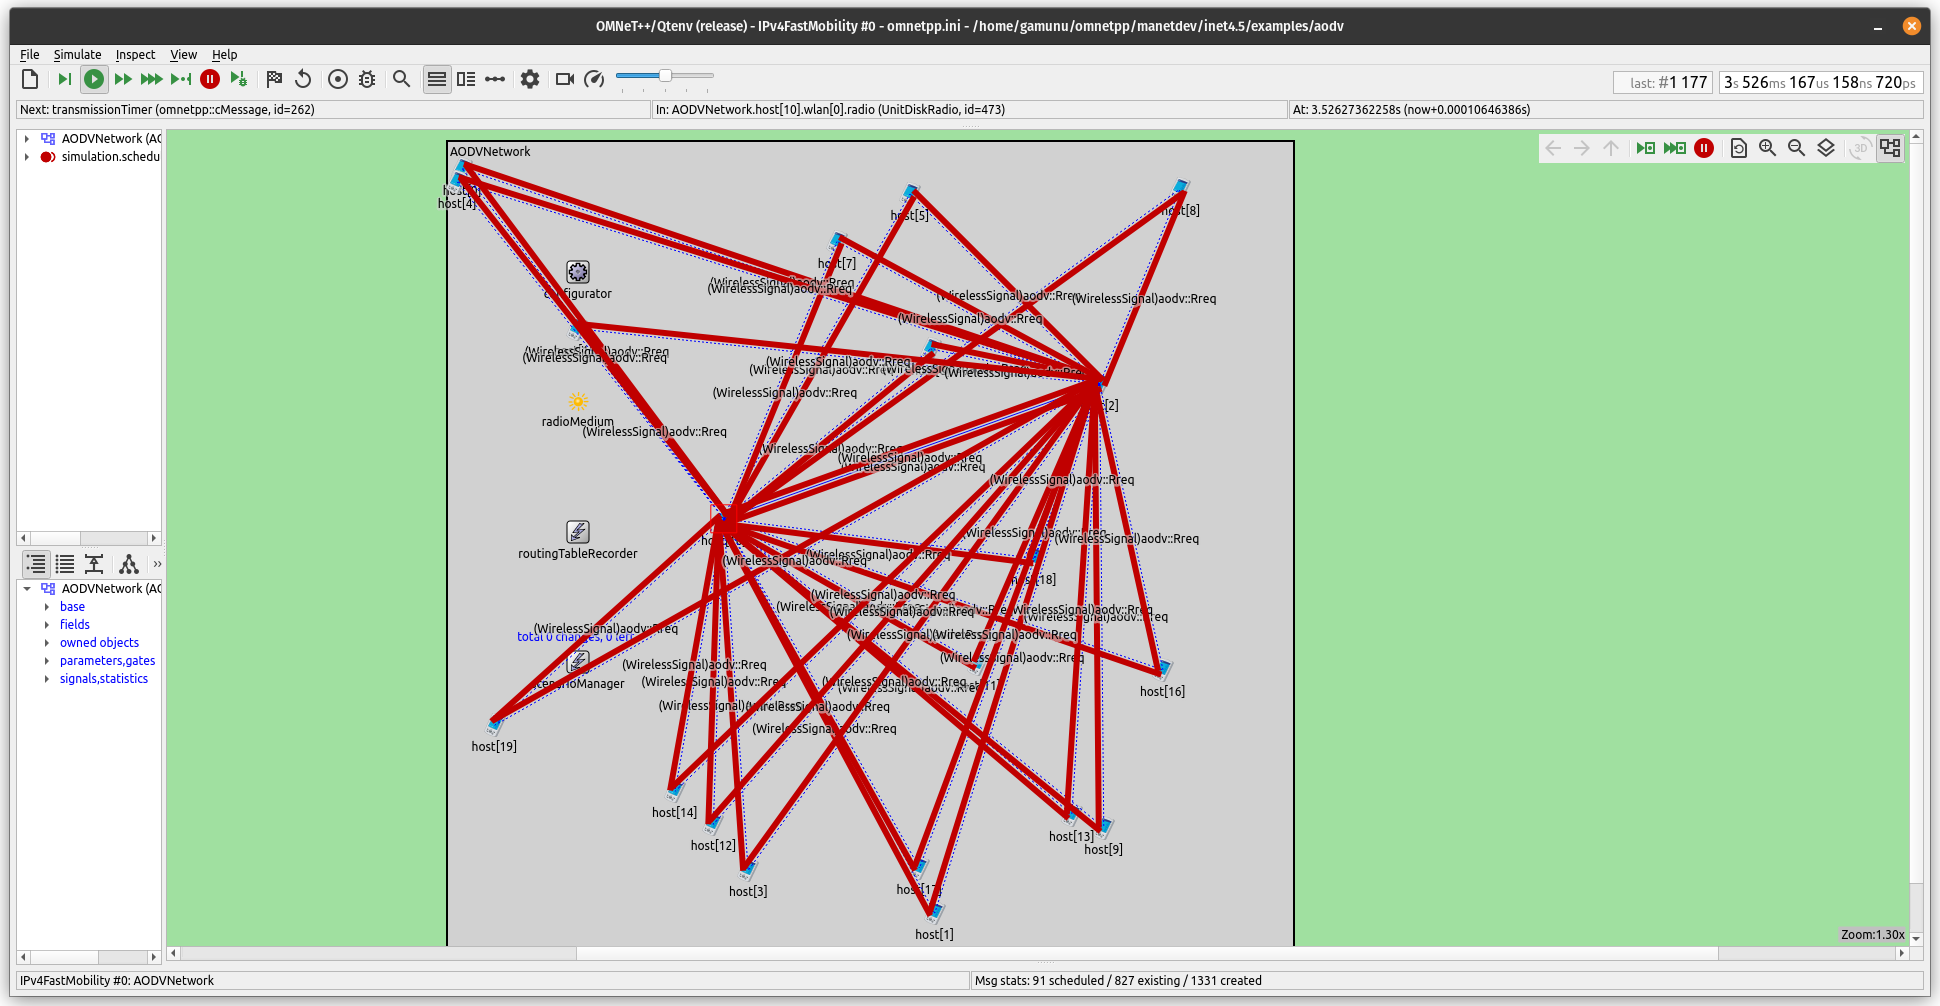
\includegraphics[height=0.45\textwidth]{imgs/aodvSim.png}}
    \caption{AODV protocol network simulation}
    \label{aodvSim}
\end{figure}

\subsubsection{WiFi Direct POC}

To test the feasibility and refine the implementation method, we have developed
a POC application for using WiFi Direct as a communication method. Currently,
communication among clients of the same group is implemented. The group
formation is handled by \texttt{WifiP2pManager}, provided by the Android
SDK\cite{wifiman}.

\vspace{0.3cm}

\paragraph{POC App Implementation}

The POC application sets up a WiFi Direct group and, once the group is
established, allows sending text messages within the created group, both
between Group Members and between Group Owner and Group Members.

The figure~\ref{labelewifidipoc} shows a labled interface of the developed POC
application.

\begin{figure}[htbp]

    \centerline{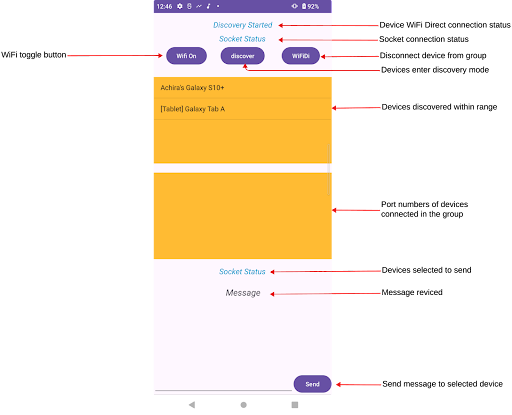
\includegraphics[height=0.9\textwidth]{imgs/labledwifidipoc.png}}
    \caption{Labled interface of the POC application.}
    \label{labelewifidipoc}
\end{figure}

Once the nearby WiFi Direct-enabled devices are discovered, the devices perform
a group owner negotiation and establish a WiFi Direct group. Once the group is
established, the Group Owner(GO or Host, as referred to in the POC application)
can communicate with the sockets connected to each device in the group.

Once this stage is reached, each client can view the host or Group Owner's
device name in the discovery list. The group owner can view the clients
connected to it. This is demonstrated in Figure~\ref{group}.

\begin{figure}
    \centering
    \begin{subfigure}[b]{0.3\textwidth}
        \includegraphics[width=\textwidth,
            height=0.4\textheight]{imgs/hostaftergroup.png}
        \caption{Host interface after creating a group with one client.}
        \label{group:host}
    \end{subfigure}
    \hspace{1cm}
    \begin{subfigure}[b]{0.3\textwidth}
        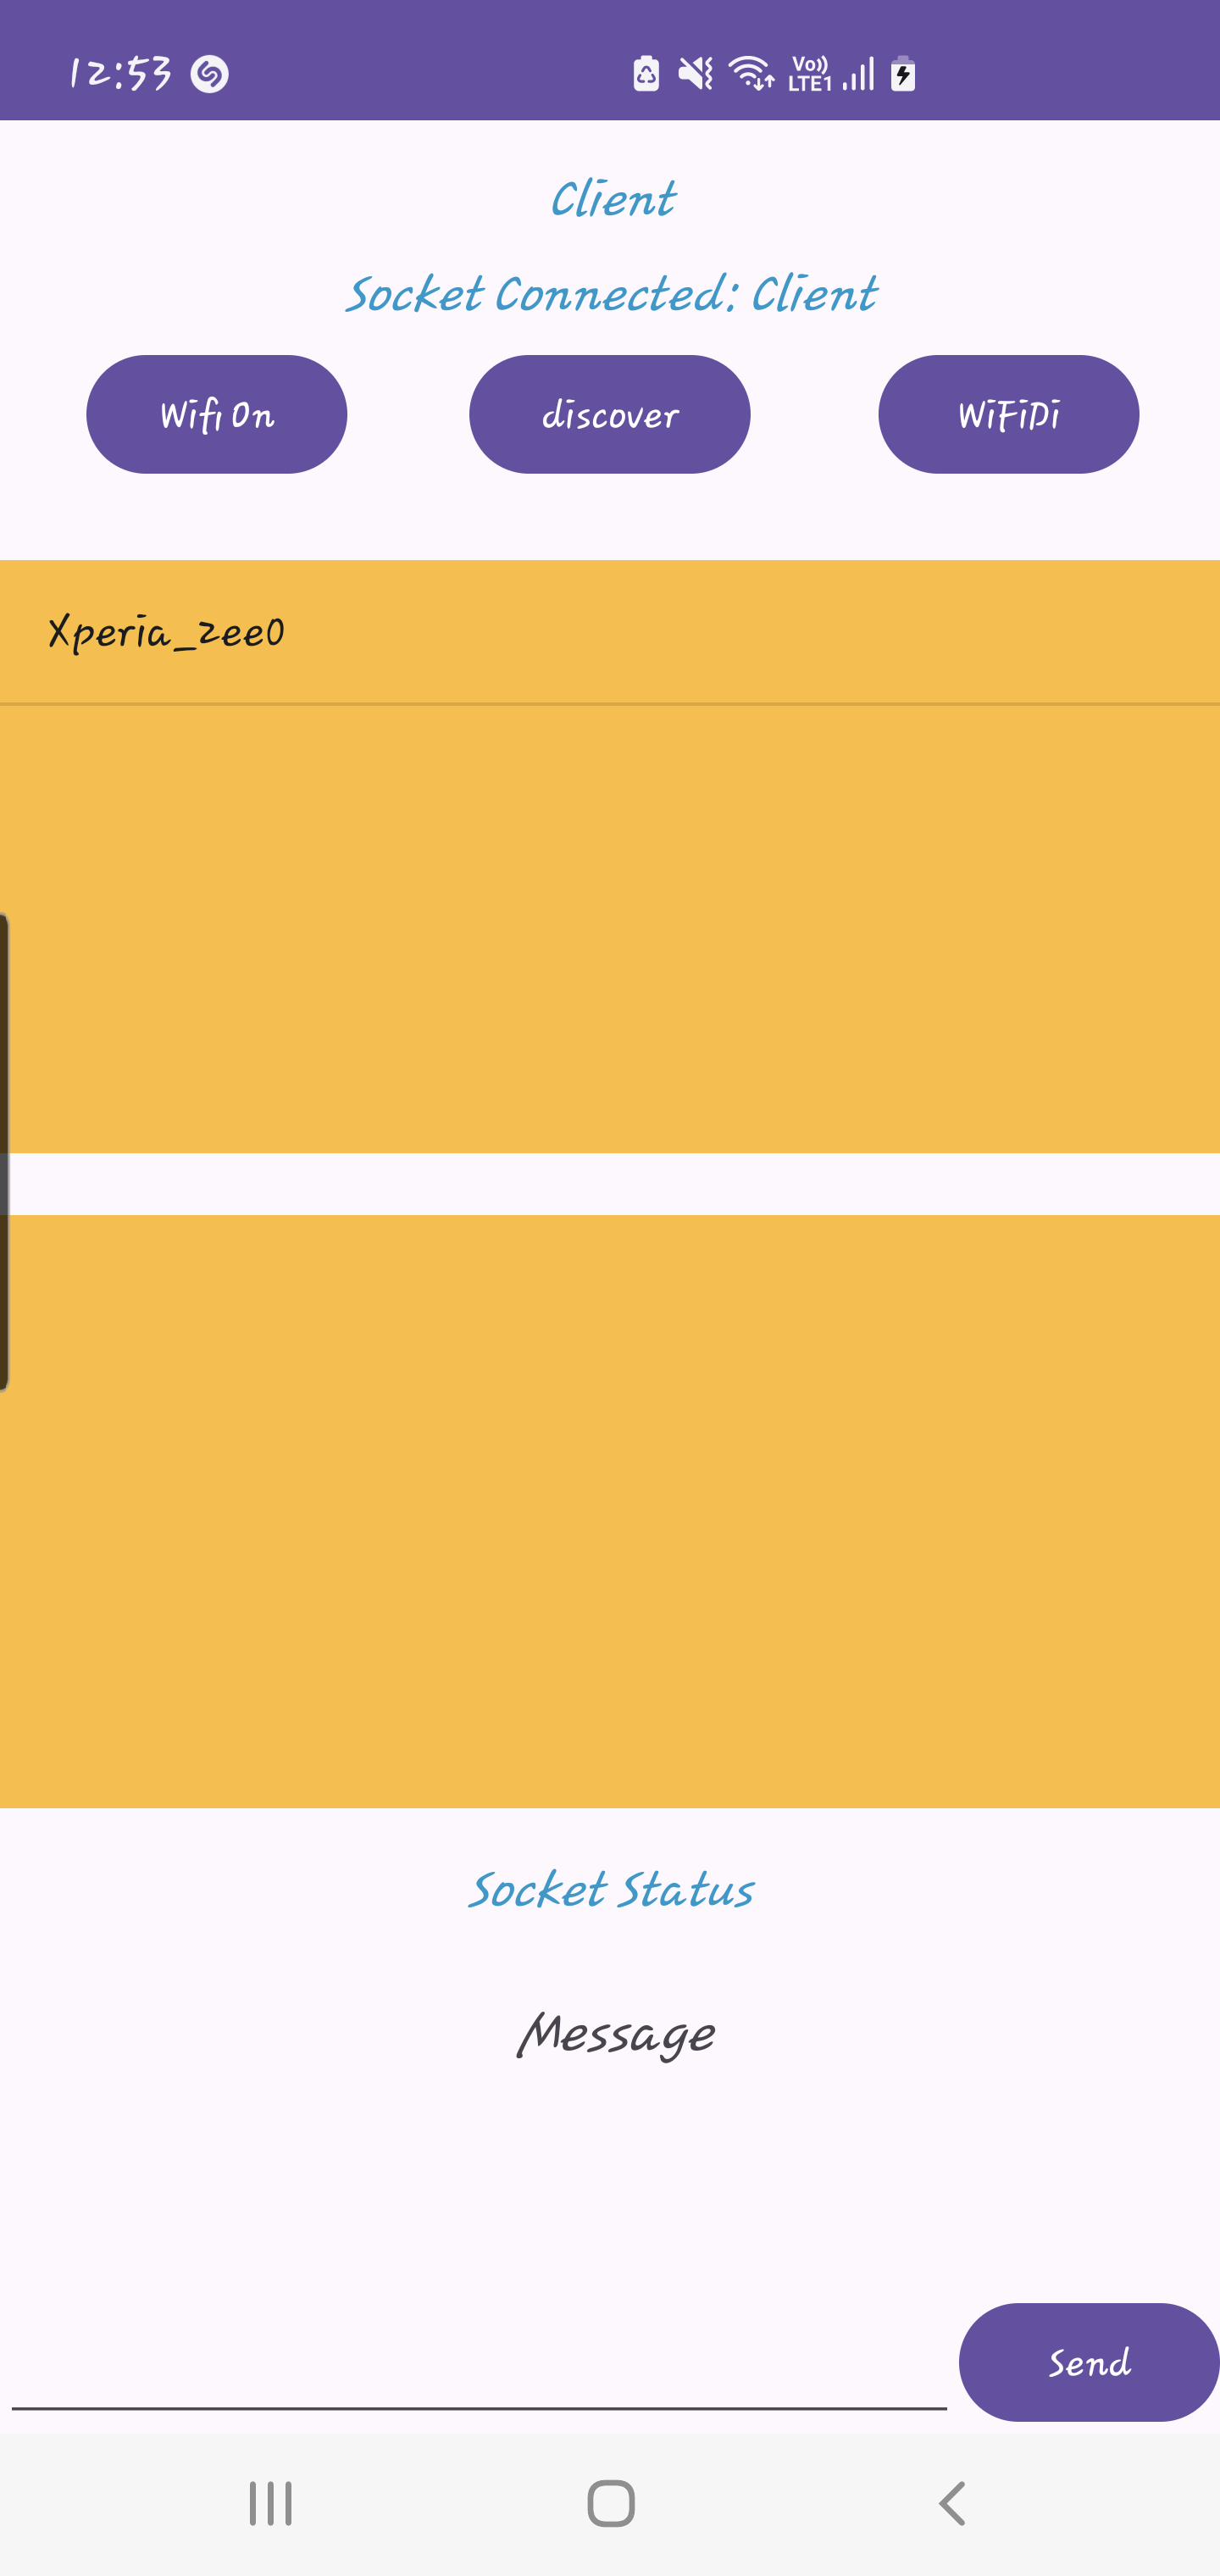
\includegraphics[width=\textwidth,
            height=0.4\textheight]{imgs/clientAfterDiscovery.png}
        \caption{Client interface after a group is created.}
        \label{group:client}
    \end{subfigure}
    \caption{Caption for the whole figure.}
    \label{group}
\end{figure}

After a group is created, communication between the host and client are
possible as demonstrated by the Figures~\ref{clientComm} and~\ref{hostComm}.

\begin{figure}
    \centering
    \begin{subfigure}[b]{0.3\textwidth}
        \centerline{
            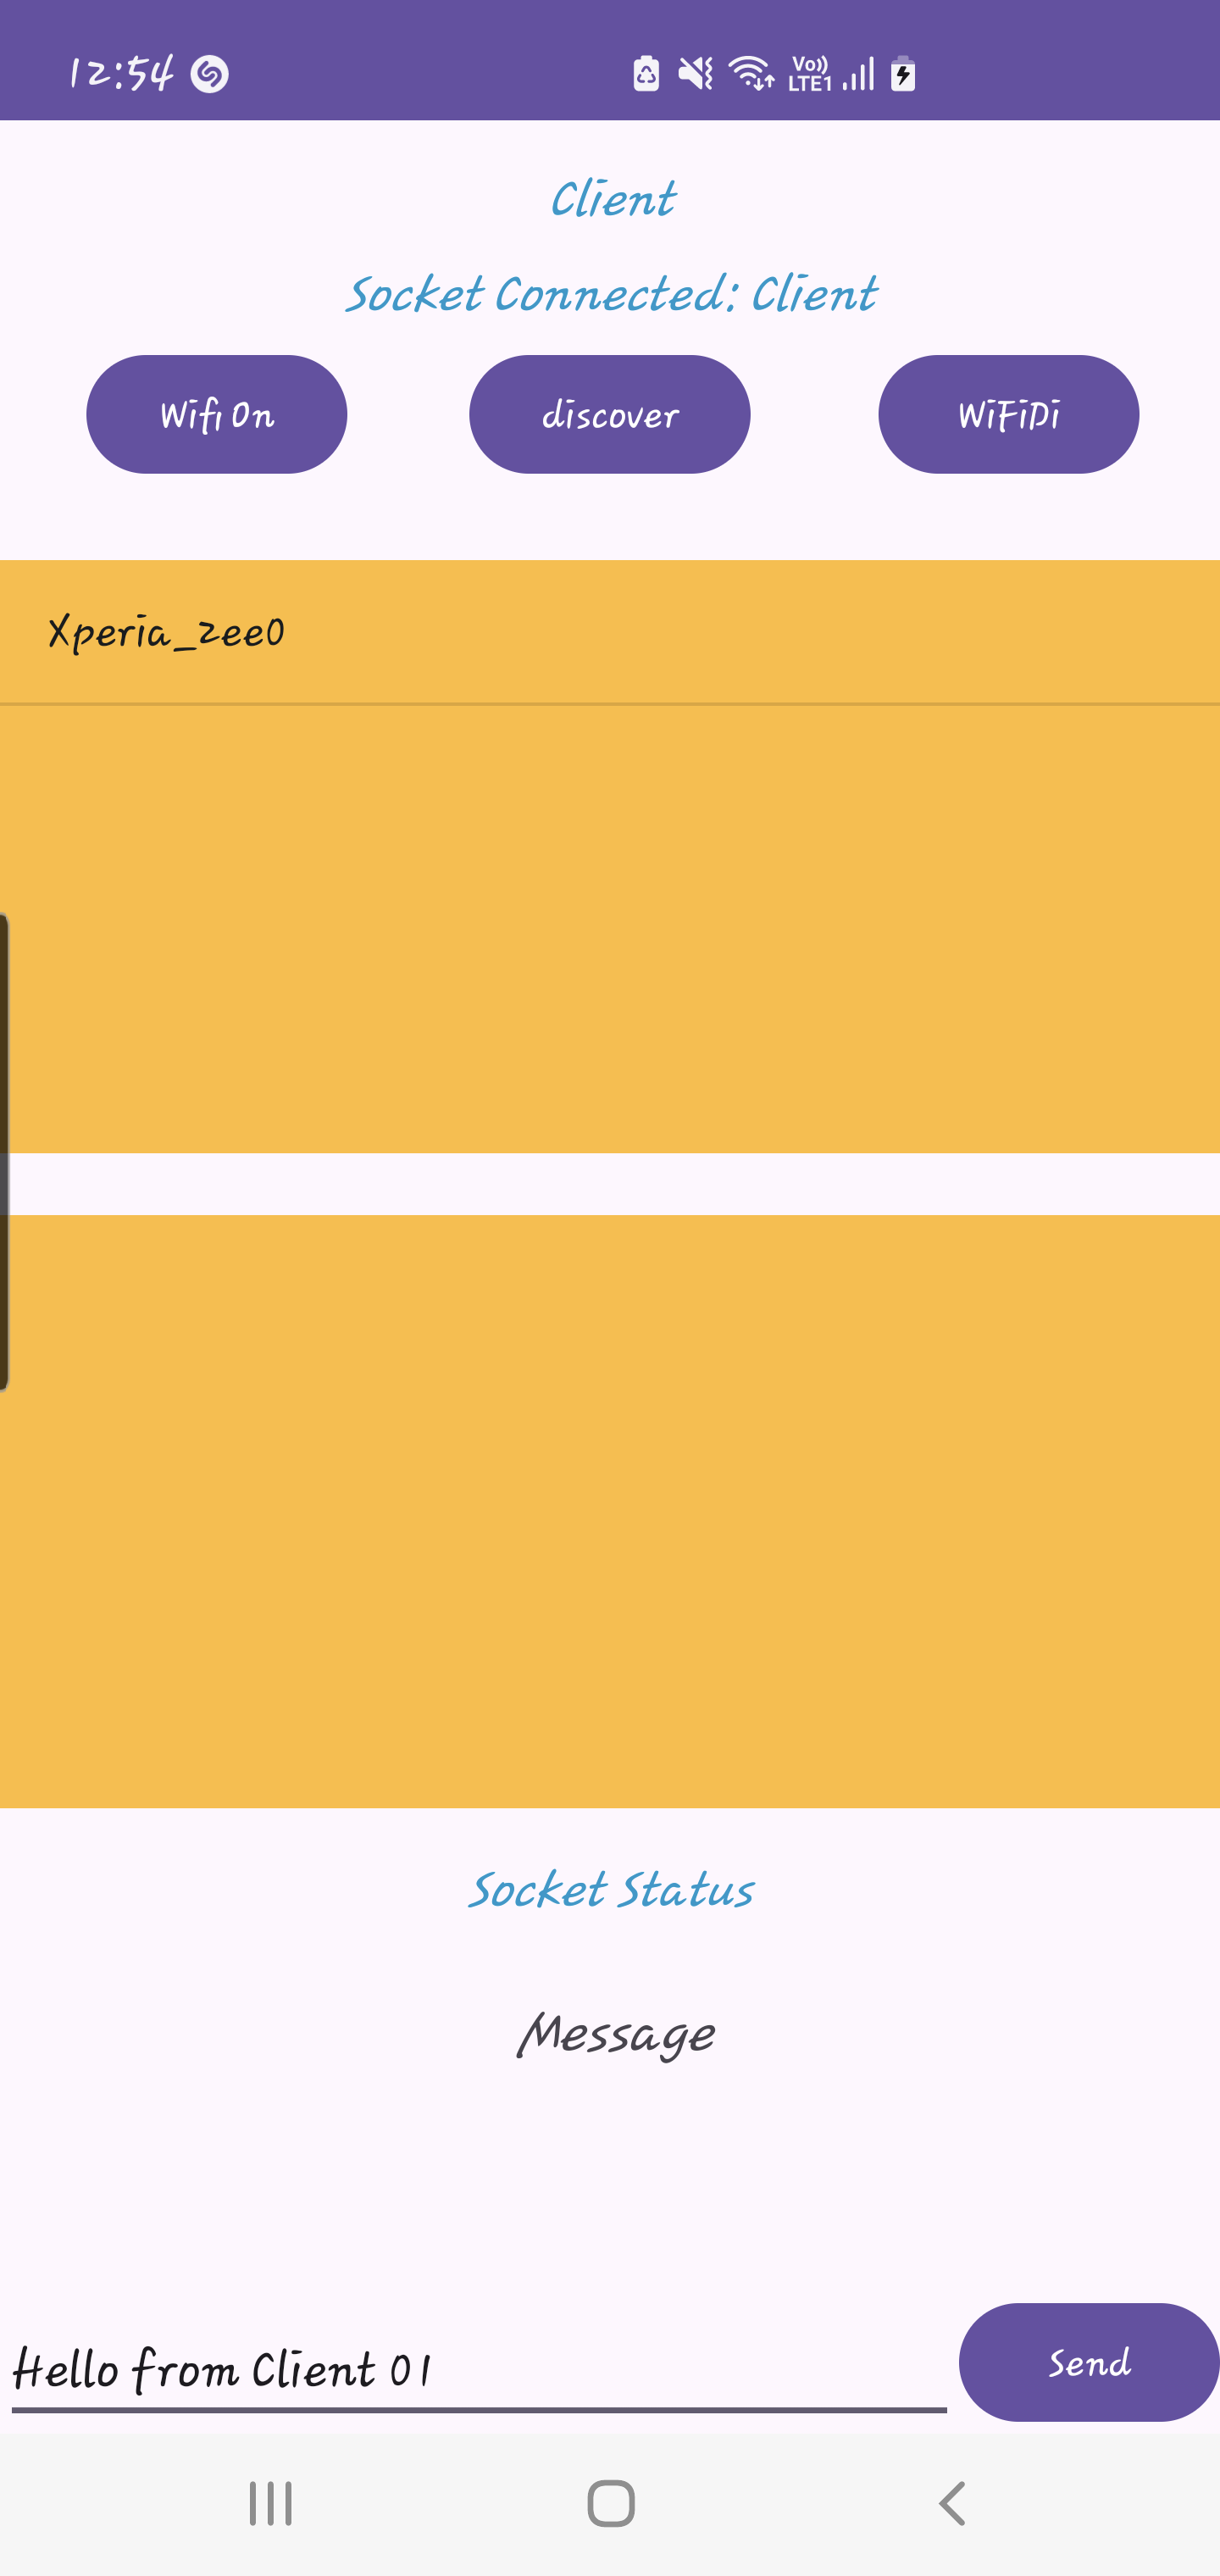
\includegraphics[width=\textwidth,
                height=0.4\textheight]{imgs/client2host-client.png}}
        \caption{Client sends a message to host.}
        \label{clientComm:c}
    \end{subfigure}
    \hspace{1cm}
    \begin{subfigure}[b]{0.3\textwidth}
        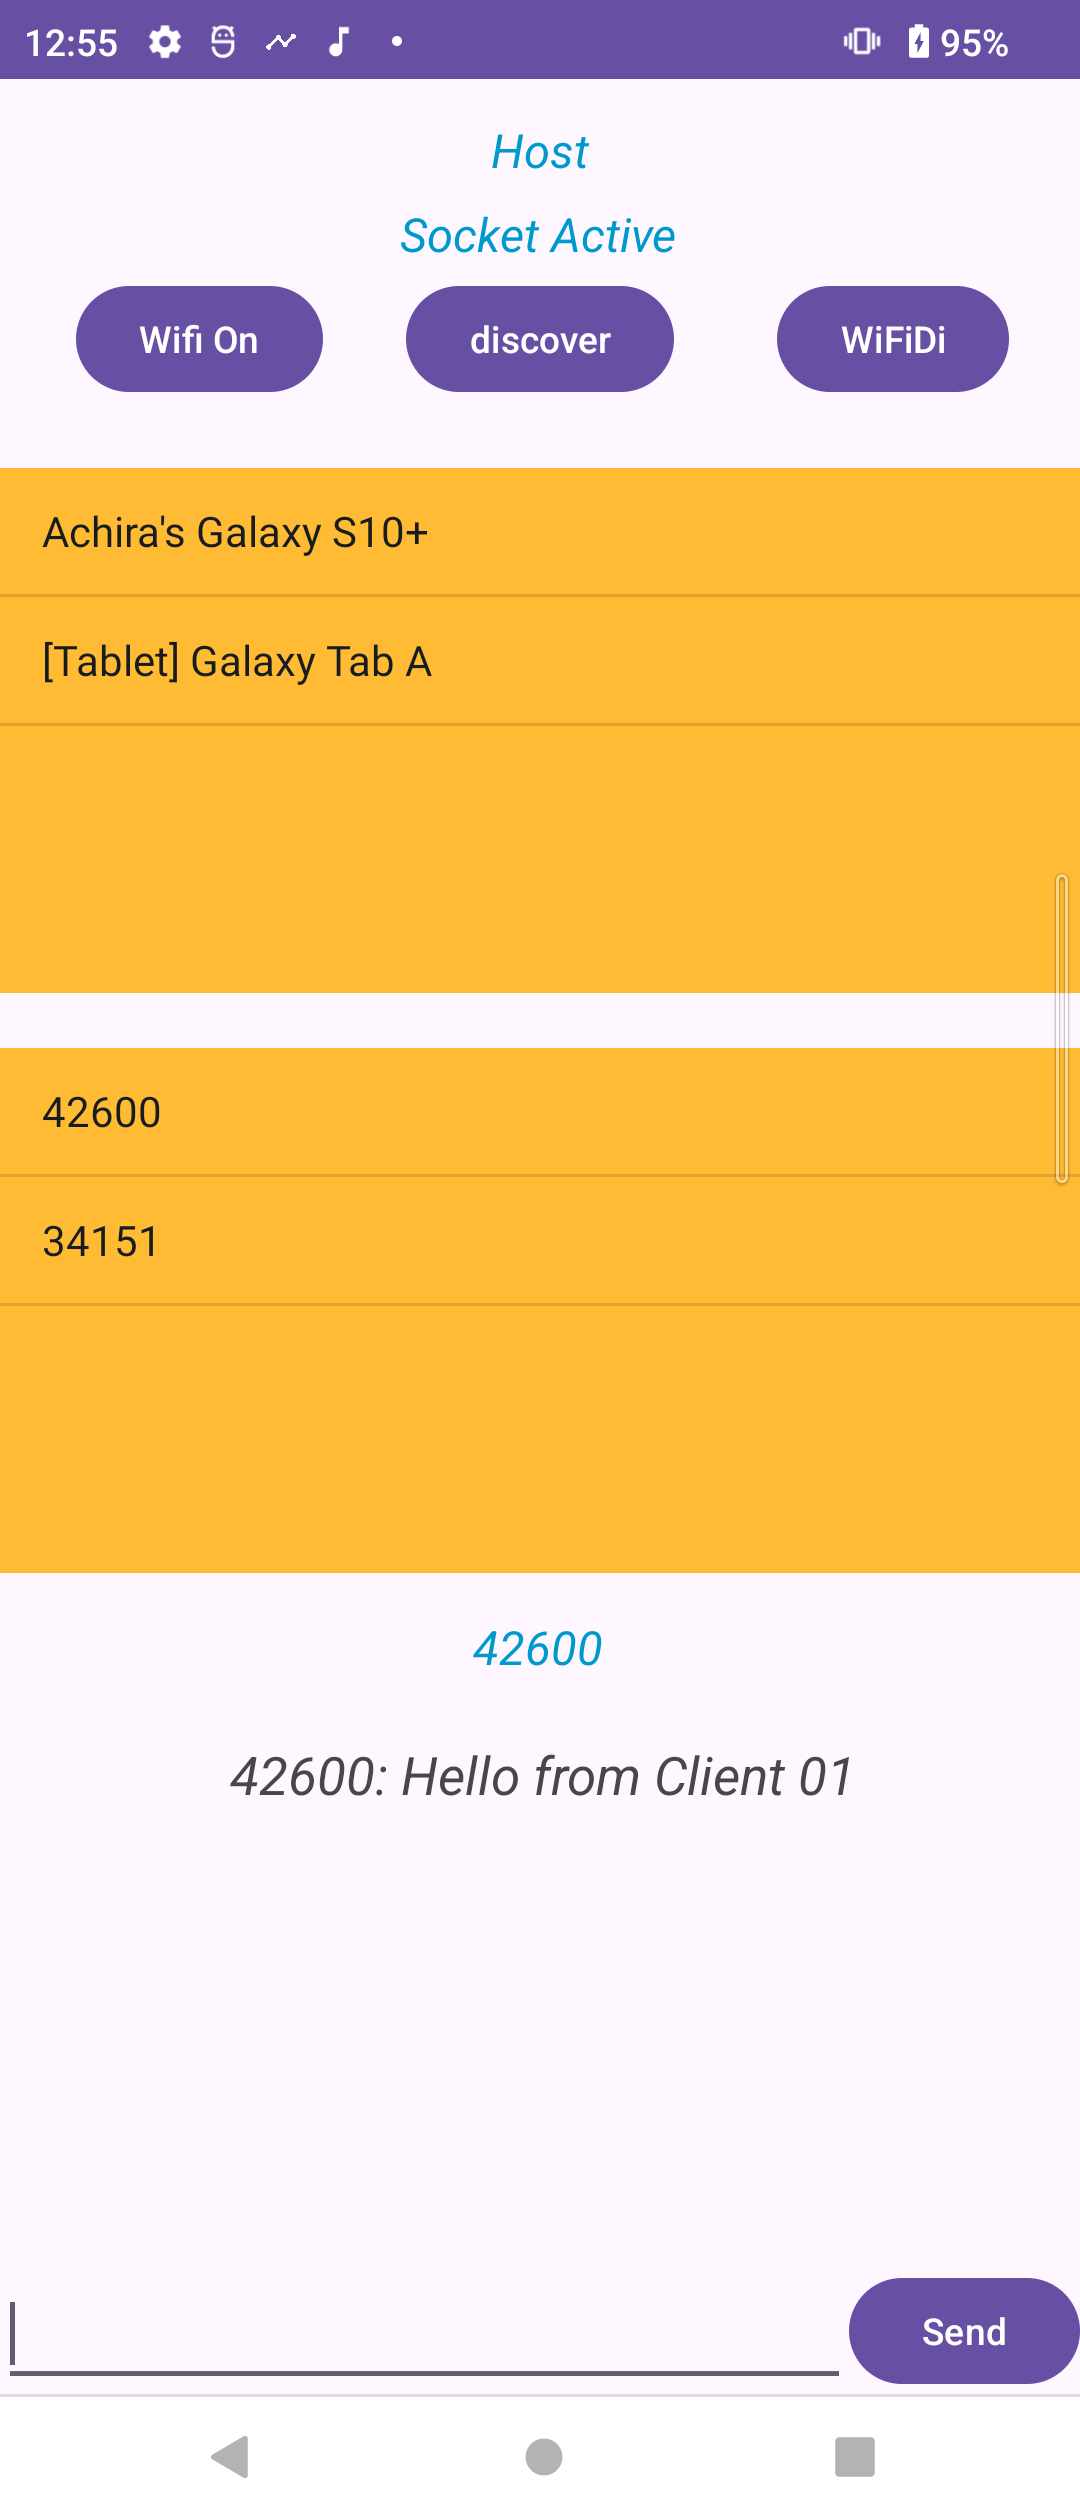
\includegraphics[width=\textwidth,
            height=0.4\textheight]{imgs/client2host-host.png}
        \caption{Message is recieved by host.}
        \label{clientComm:h}
    \end{subfigure}
    \caption{Sending messages from Client to Host.}
    \label{clientComm}
\end{figure}

\begin{figure}
    \centering
    \begin{subfigure}[b]{0.3\textwidth}
        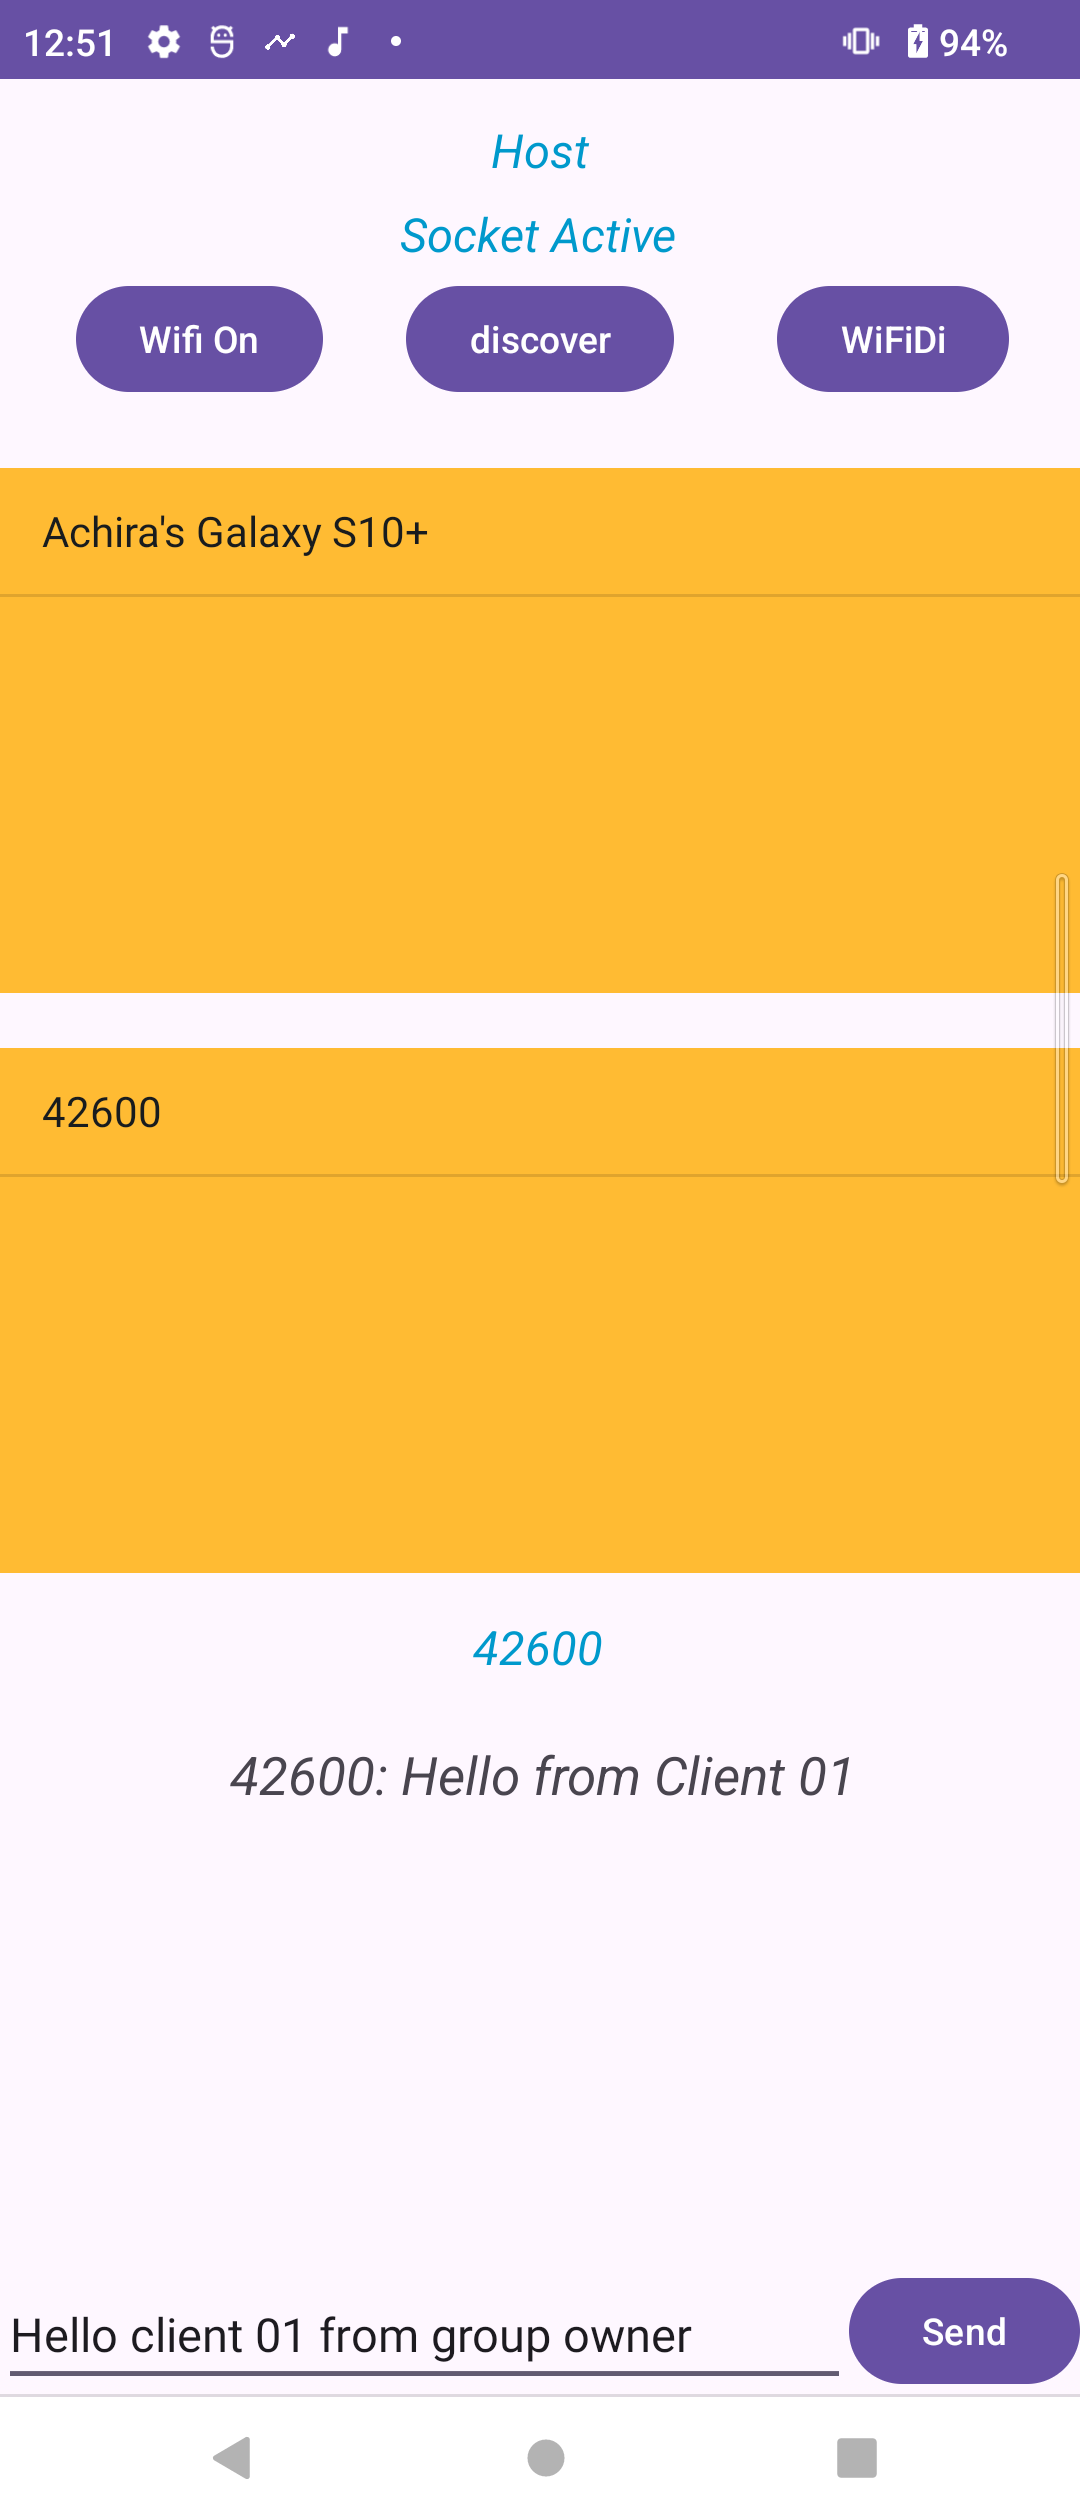
\includegraphics[width=\textwidth,
            height=0.4\textheight]{imgs/host2client-host.png}
        \caption{Host sends a message to client.}
        \label{hostComm:h}
    \end{subfigure}
    \hspace{1cm}
    \begin{subfigure}[b]{0.3\textwidth}
        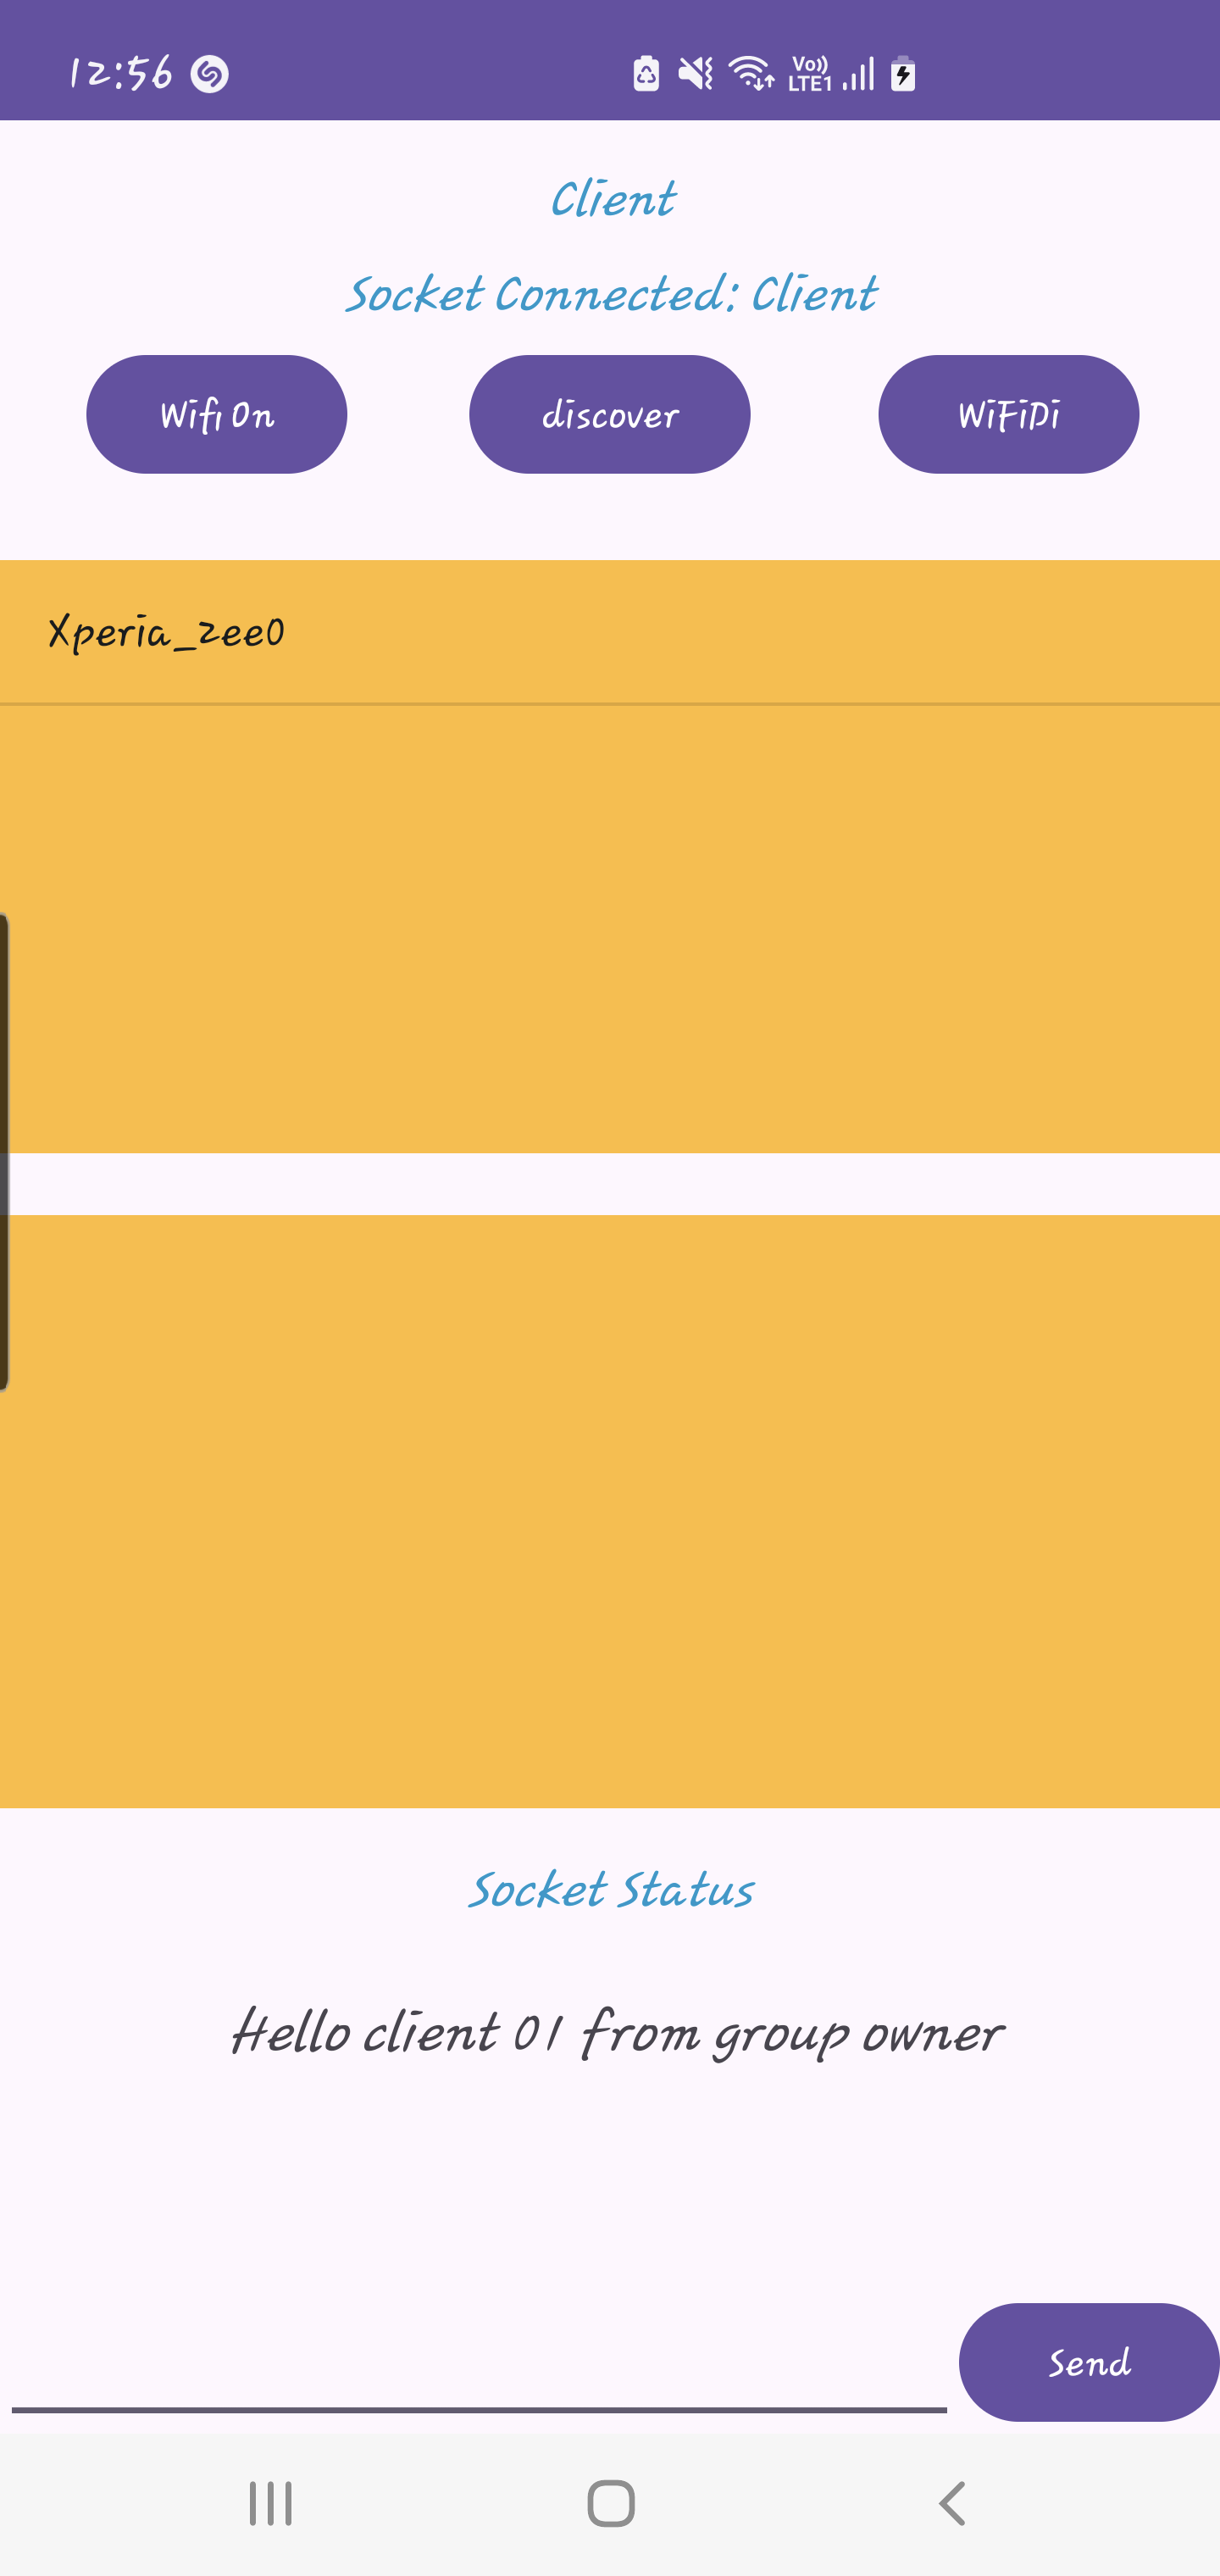
\includegraphics[width=\textwidth,
            height=0.4\textheight]{imgs/host2client-client.png}
        \caption{Message is recieved by client.}
        \label{hostComm:c}
    \end{subfigure}
    \caption{Sending messages from Host to Client.}
    \label{hostComm}
\end{figure}

It is also possible for another device to connect to an already established
Group. In such a case, the join request will be approved by the Group Owner.
This is demonstrated by the Figure~\ref{newClient}.

\begin{figure}
    \centering
    \begin{subfigure}[b]{0.6\textwidth}
        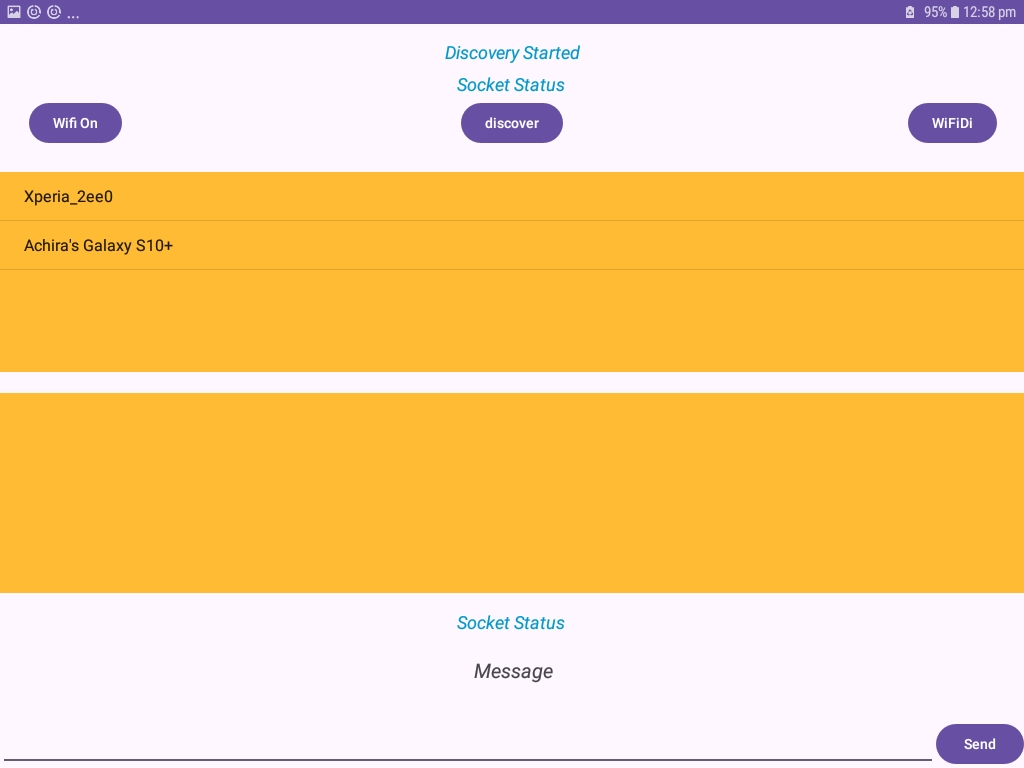
\includegraphics[width=\textwidth,
            height=0.4\textheight]{imgs/discovery-newclient.jpg}
        \caption{A new client is in discovery mode within range of the existing
            group owner}
        \label{newClient:discover}
    \end{subfigure}
    \hspace{1cm}
    \begin{subfigure}[b]{0.3\textwidth}
        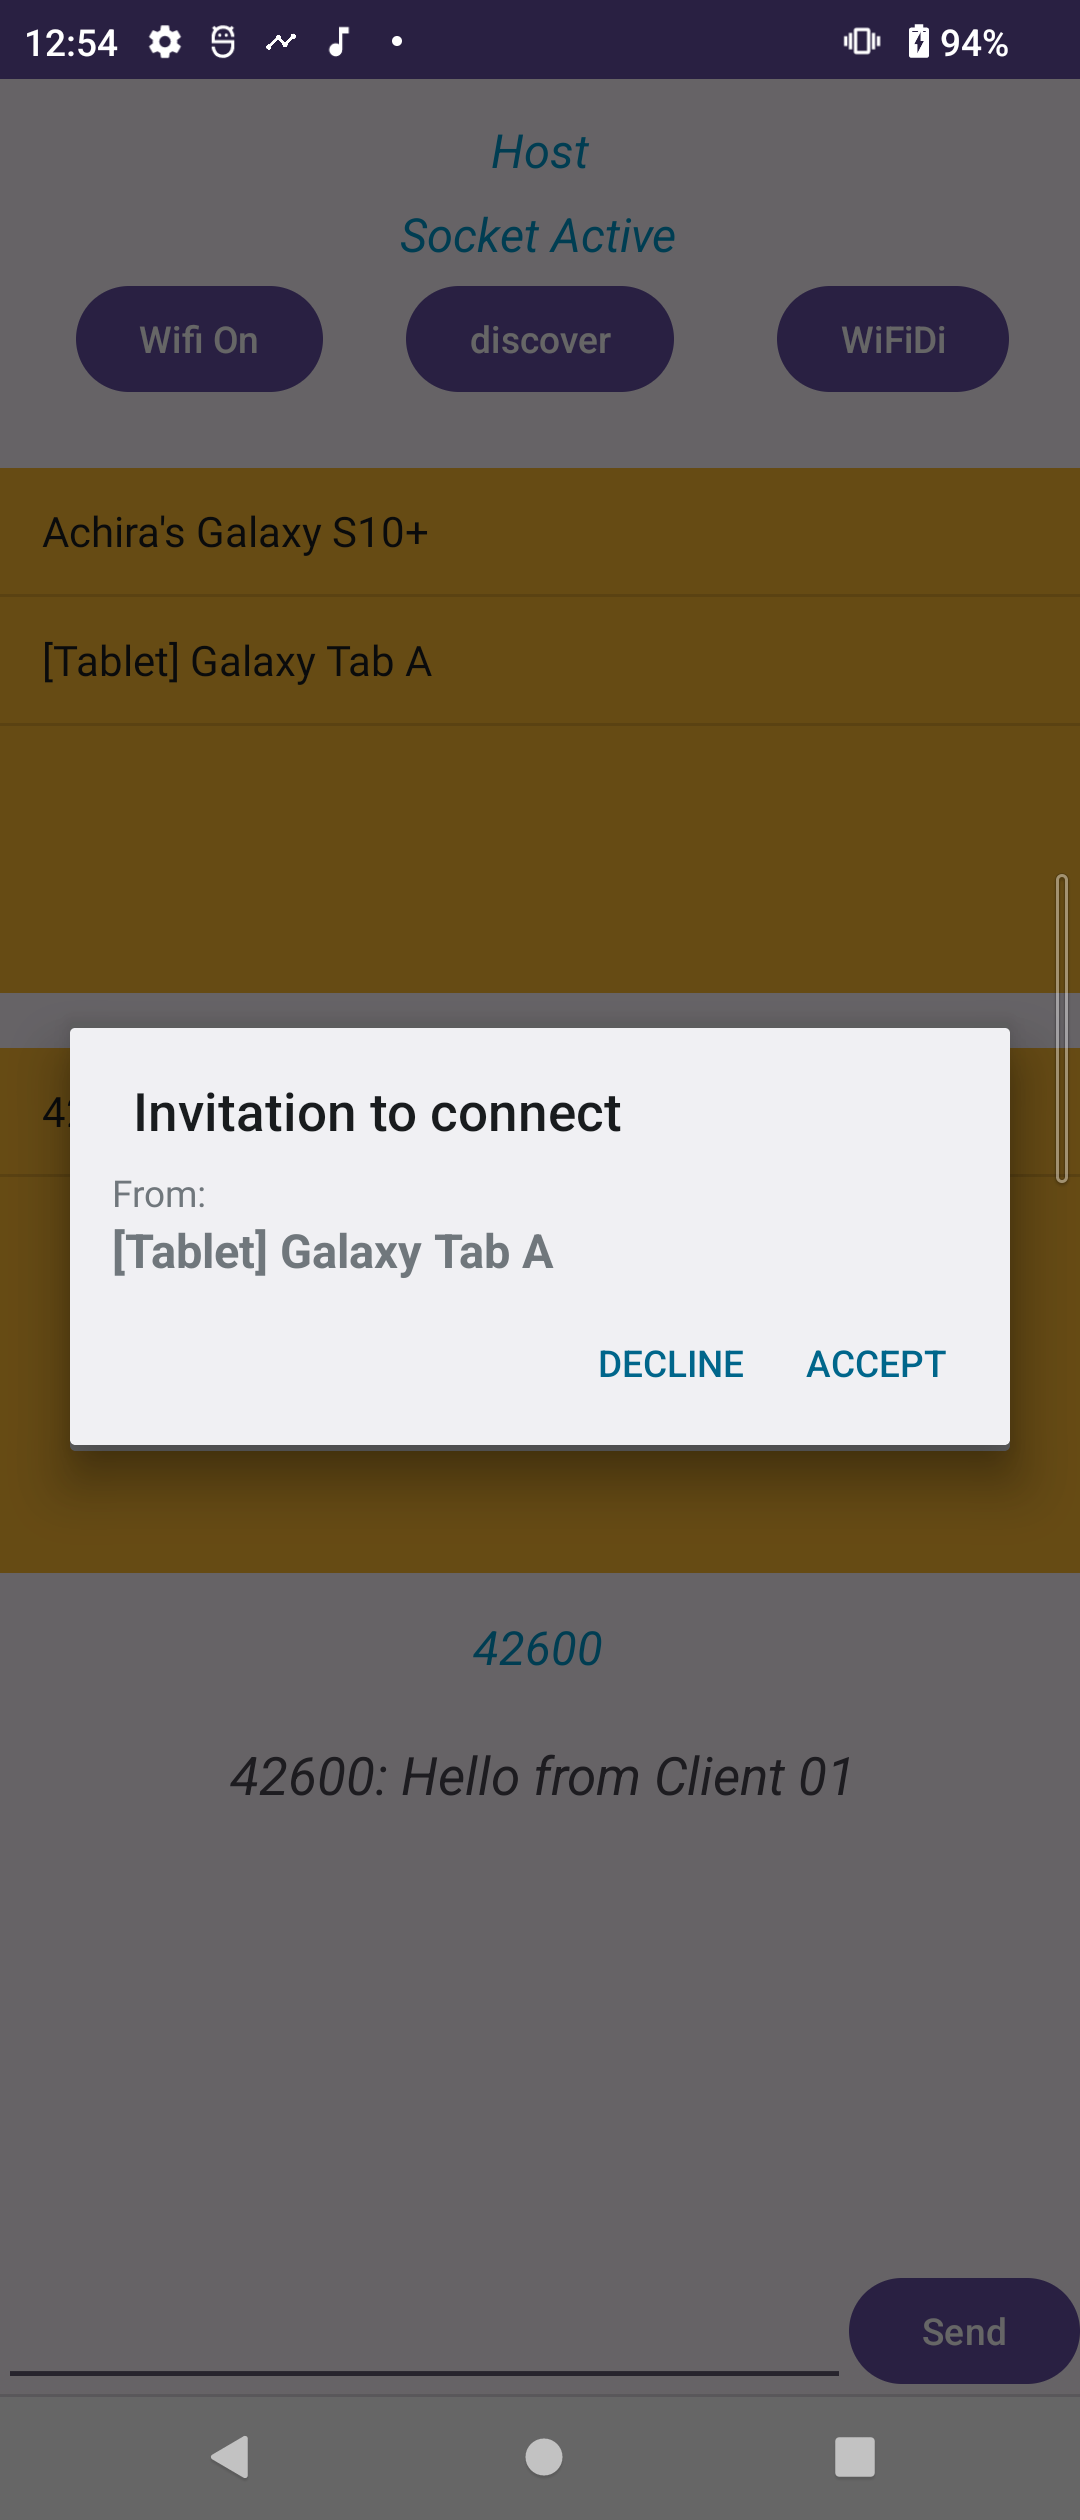
\includegraphics[width=\textwidth,
            height=0.4\textheight]{imgs/newdevice-host.png}
        \caption{Host recieves an incoming connection request from new client.}
        \label{newClient:request}
    \end{subfigure}
    \hspace{1cm}
    \begin{subfigure}[b]{0.6\textwidth}
        \includegraphics[width=\textwidth,
            height=0.4\textheight]{imgs/newClientConnected.jpg}
        \caption{The new client is connected to the group}
        \label{newClient:connected}
    \end{subfigure}
    \caption{Connecting a new client to the existing WiFiDi group}
    \label{newClient}
\end{figure}

Client to client communication is also possible. Such messages will be routed
by the Group Owner. This is demonstrated by Figure~\ref{c2c}.

\begin{figure}
    \centering
    \begin{subfigure}[b]{0.6\textwidth}
        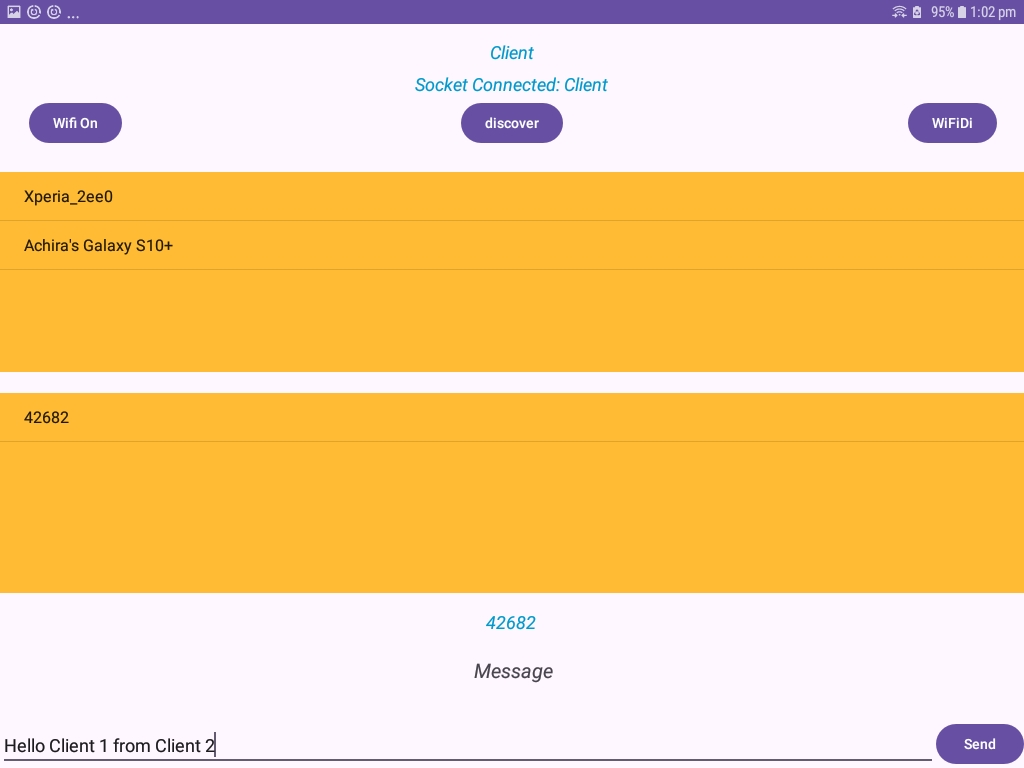
\includegraphics[width=\textwidth,
            height=0.4\textheight]{imgs/client2client-client2.jpg}
        \caption{New client sends a message to \texttt{Client 01}.}
        \label{c2c:1}
    \end{subfigure}
    \hspace{1cm}
    \begin{subfigure}[b]{0.3\textwidth}
        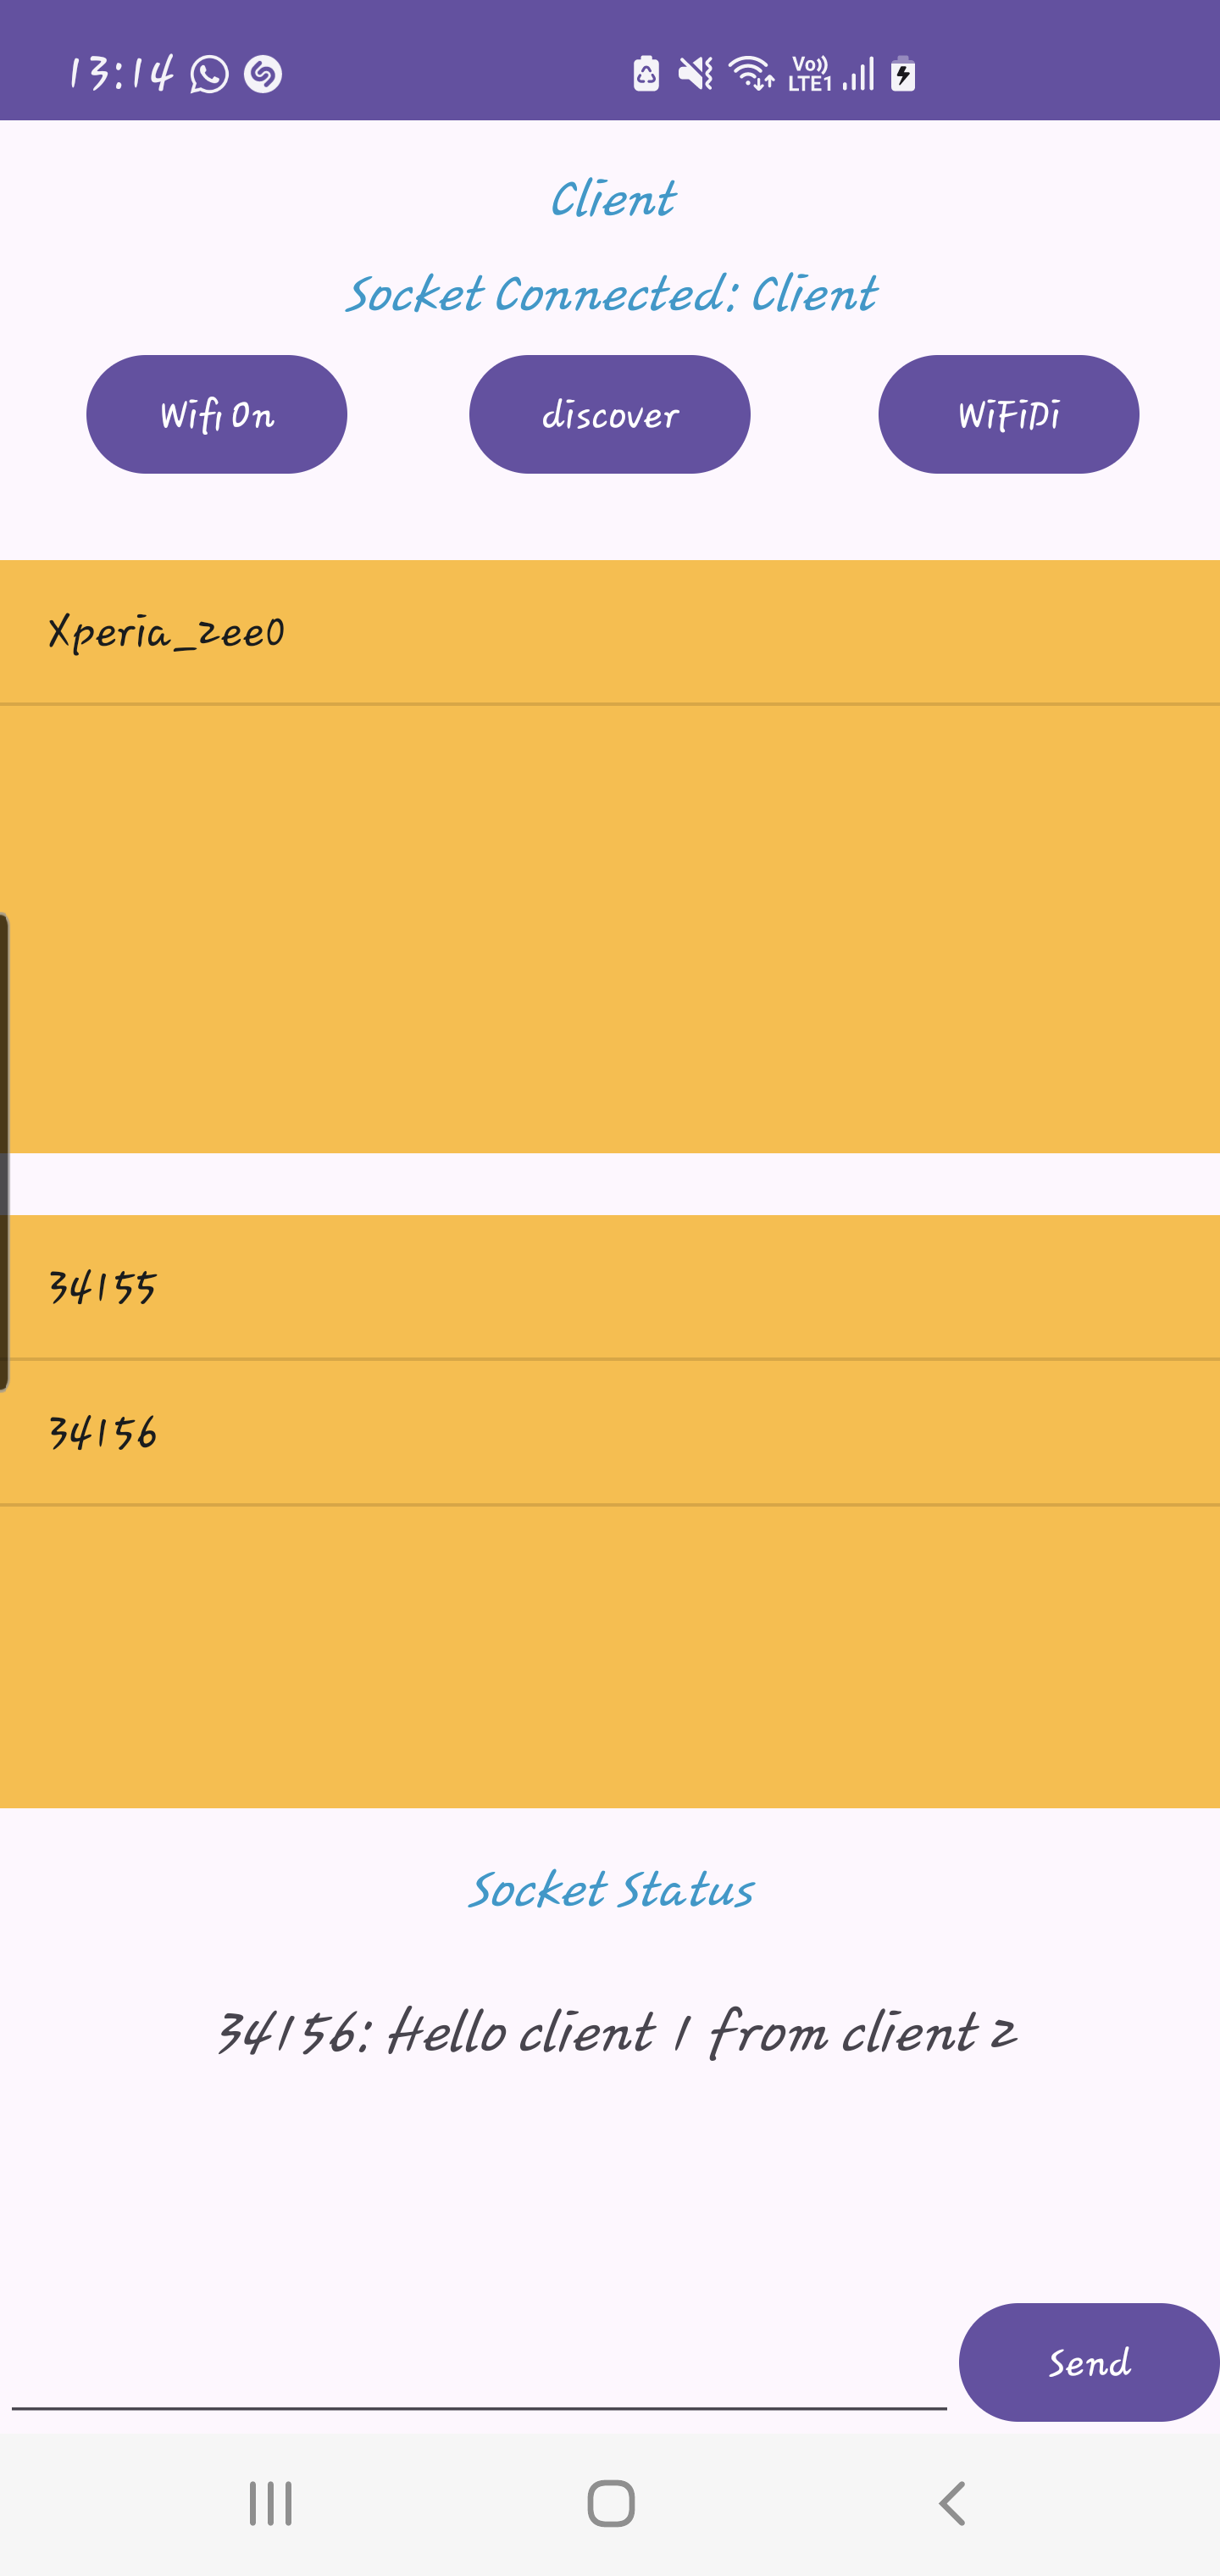
\includegraphics[width=\textwidth,
            height=0.4\textheight]{imgs/client2client-client1.png}
        \caption{Message is recieved by \texttt{Client 01}.}
        \label{c2c:2}
    \end{subfigure}
    \caption{Sending messages from Client to Client.}
    \label{c2c}
\end{figure}

\subsubsection{Improving the framework from Meshify}

Previously the app and the Meshify framework were built in the same project.
Built the framework as a different library project from scratch based on the
previous Meshify framework. The framework supports Bluetooth and BLE.
Framework mainly consists of three sections which are API, Controller and the
Entity. API consists of the main APIs for the framework, Controller consists of
the logic behind the framework where all the above-discussed techniques
including the flooding mechanism with TARP are implemented and Entity
constitutes the foundation for data representation and manipulation within the
Meshify framework. The framework is reusable and modular, allowing its
integration into different applications. All the classes and functionalities of
the framework have been documented for clarification and ease of use.

\vspace{0.3cm}

\subsubsection{Test App for Bluetooth and BLE}

The test app designed to evaluate the framework revealed successful performance
across the following Bluetooth functionalities:

\begin{itemize}
    \item Direct messaging
    \item Multi-hop messaging
    \item Broadcast messaging
\end{itemize}

\begin{figure}
    \centering
    \begin{subfigure}[b]{0.3\textwidth}
        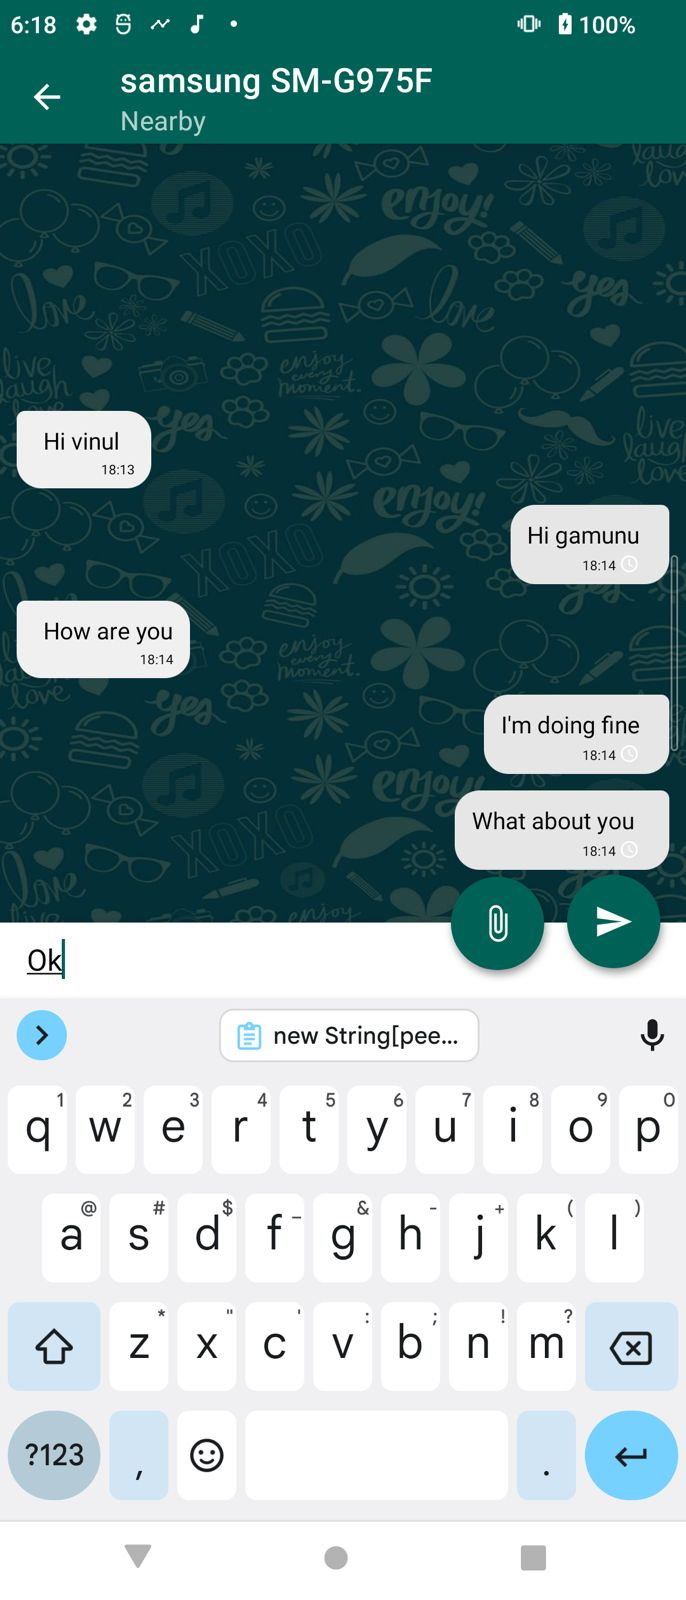
\includegraphics[width=\textwidth,
            height=0.4\textheight]{imgs/dm1.jpeg}
        %\caption{New client sends a message to \texttt{Client 01}.}
        \label{dm:1}
    \end{subfigure}
    \hspace{1cm}
    \begin{subfigure}[b]{0.3\textwidth}
        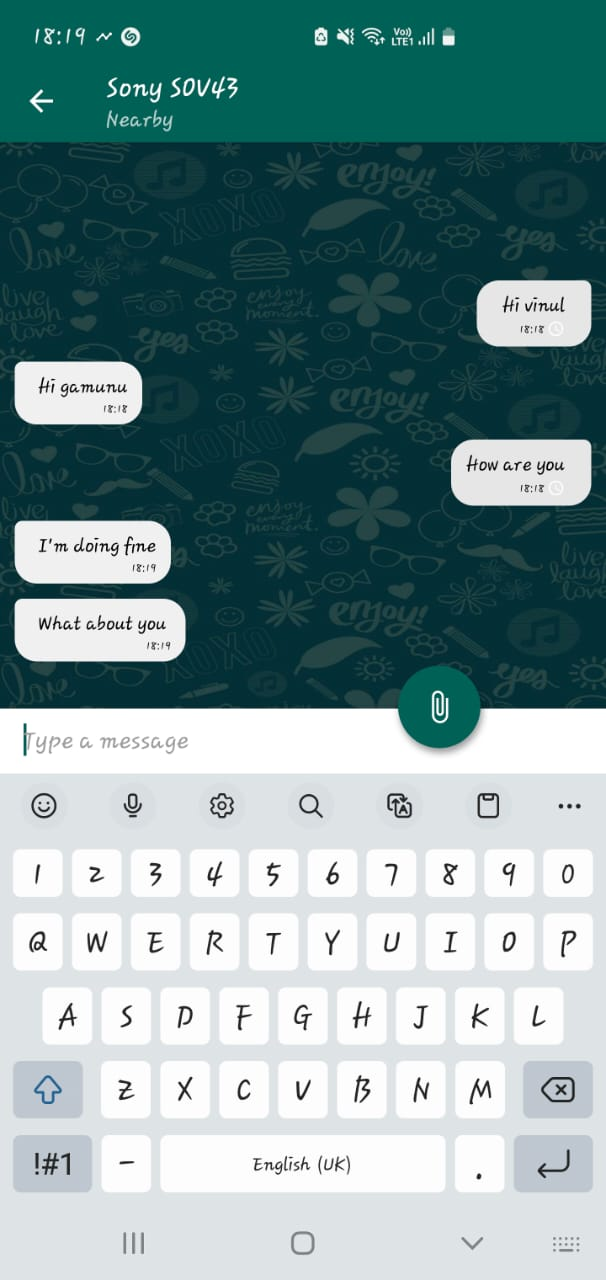
\includegraphics[width=\textwidth,
            height=0.4\textheight]{imgs/dm2.jpeg}
        %\caption{Message is recieved by \texttt{Client 01}.}
        \label{dm:2}
    \end{subfigure}
    \caption{A direct message conversation among two devices.}
    \label{dm}
\end{figure}

\begin{figure}
    \centering
    \begin{subfigure}[b]{0.3\textwidth}
        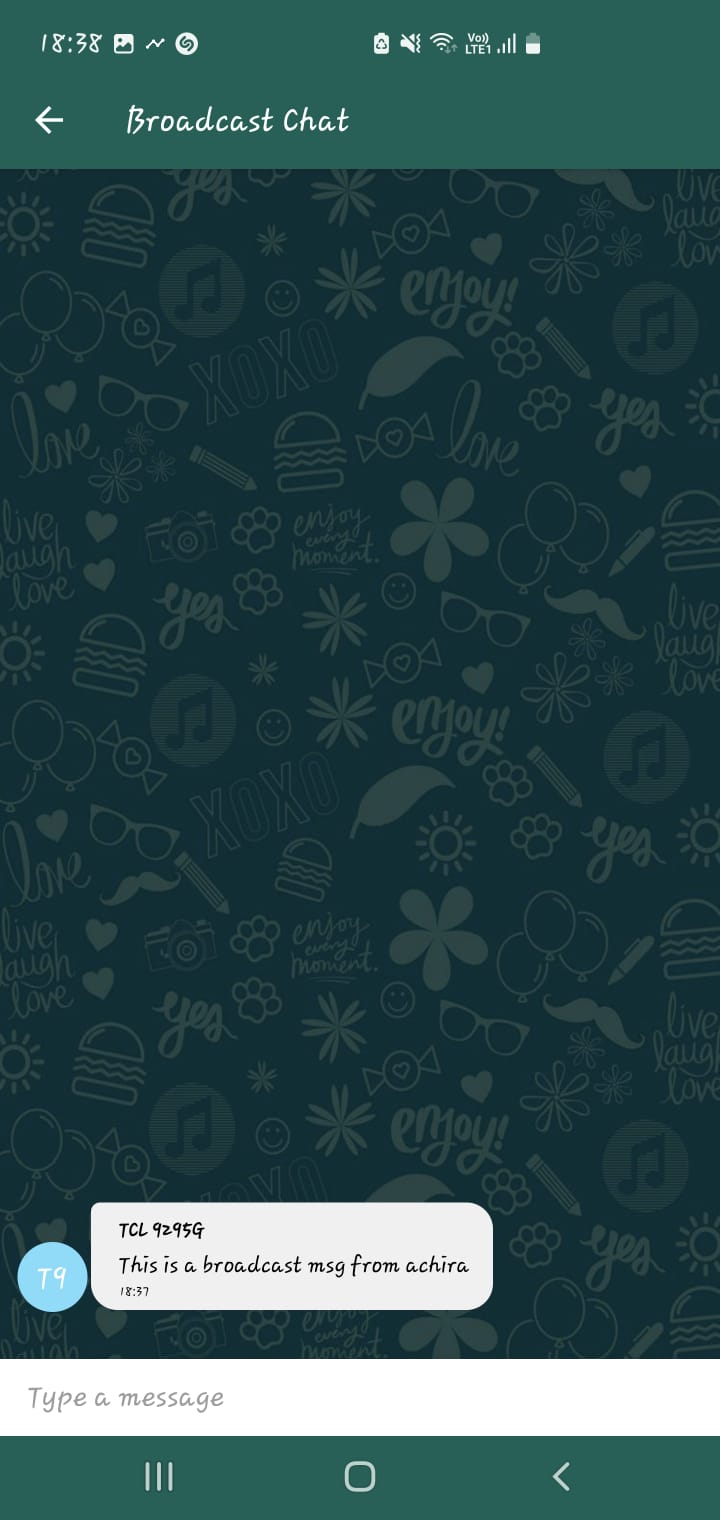
\includegraphics[width=\textwidth,
            height=0.4\textheight]{imgs/broad1.jpeg}
        %\caption{New client sends a message to \texttt{Client 01}.}
        \label{broad:1}
    \end{subfigure}
    \hspace{1cm}
    \begin{subfigure}[b]{0.3\textwidth}
        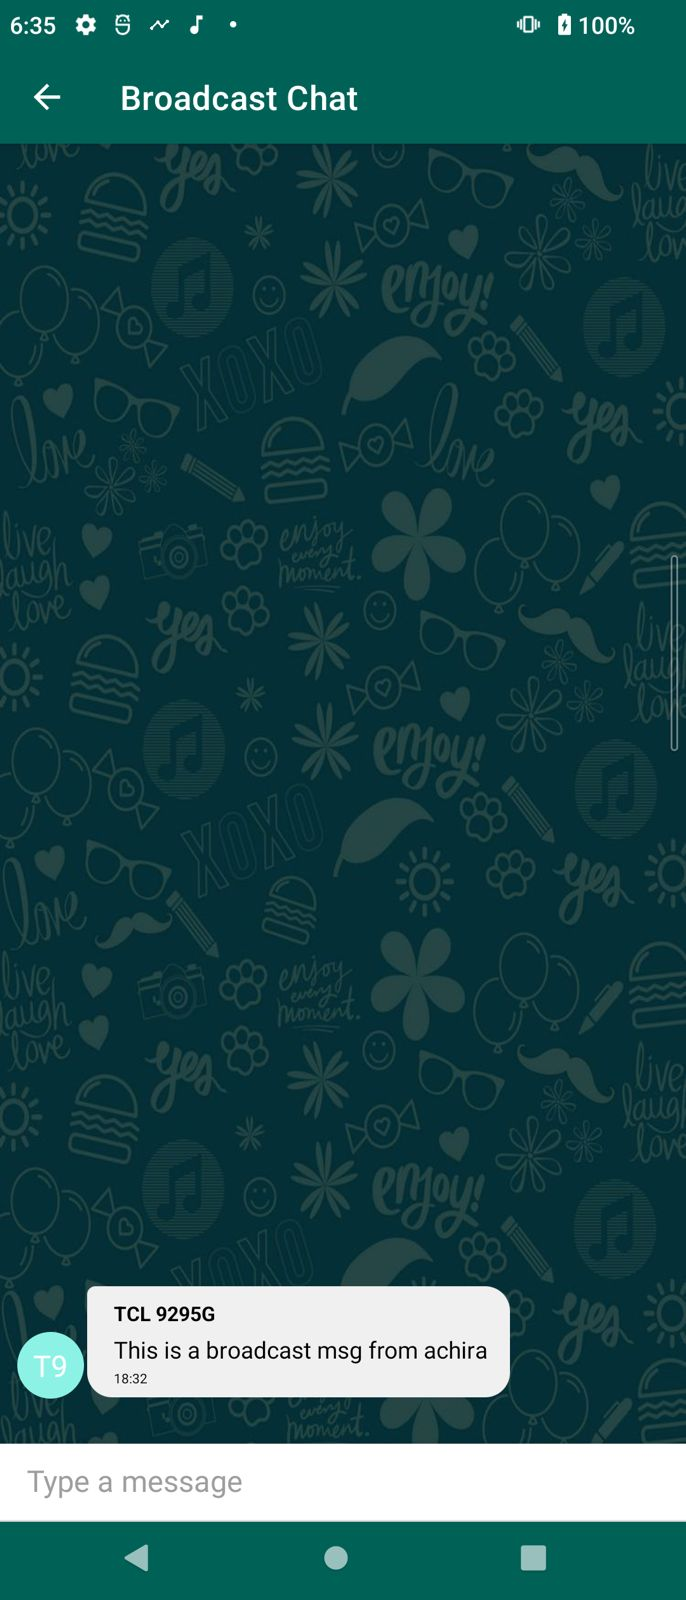
\includegraphics[width=\textwidth,
            height=0.4\textheight]{imgs/broad2.jpeg}
        %\caption{Message is recieved by \texttt{Client 01}.}
        \label{broad:2}
    \end{subfigure}
    \hspace{1cm}
    \begin{subfigure}[b]{0.4\textwidth}
        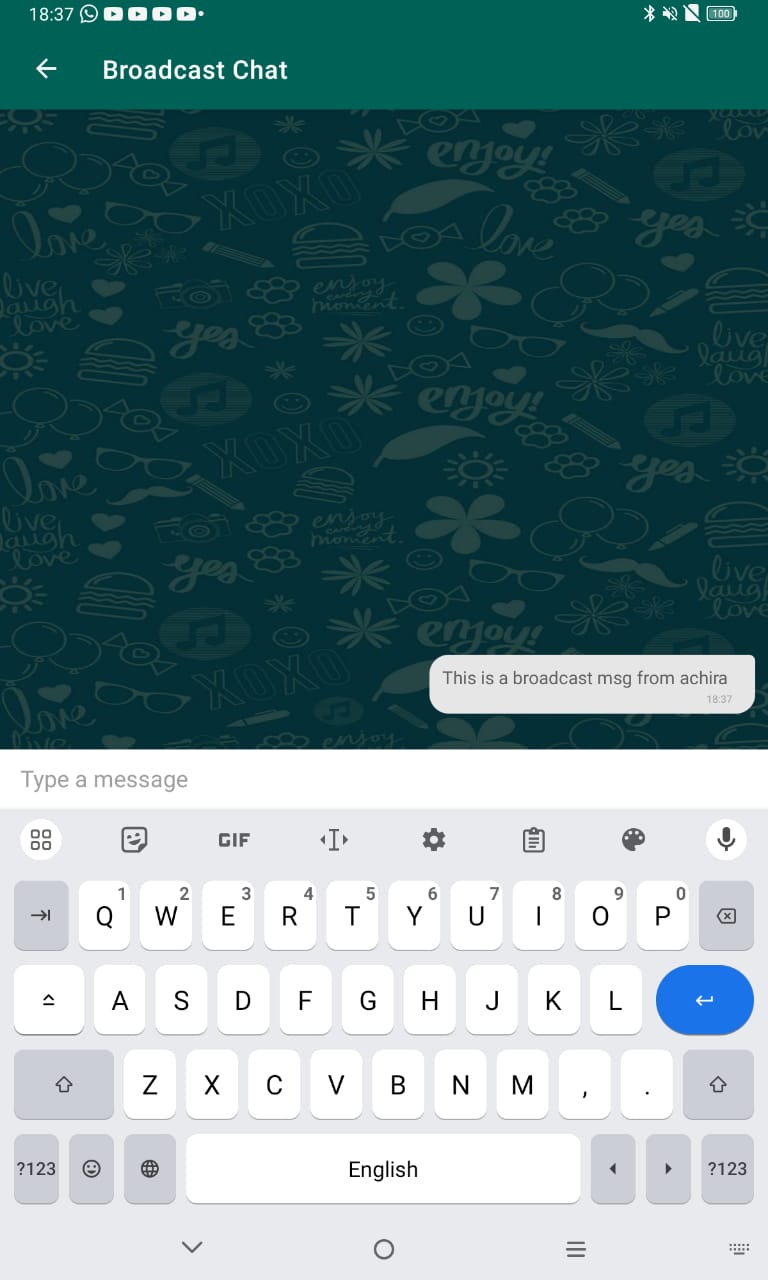
\includegraphics[width=\textwidth,
            height=0.4\textheight]{imgs/broad3.jpeg}
        %\caption{Message is recieved by \texttt{Client 01}.}
        \label{broad:3}
    \end{subfigure}
    \caption{Three deviced in broadcast messaging.}
    \label{broad}
\end{figure}

Figure~\ref{dm} demonstrates the direct messaging function.
Figure~\ref{broad} demonstrates the broadcast messaging function.

\newpage

\subsection{Upcoming Work}

\subsubsection{Simulation}
\begin{itemize}
    \item Completing the TARP protocol implementation
    \item Performing simulations and analysing data to evaluate relative
          efficiencies of the protocols.
    \item Reporting simulation results in a suitable publication medium.
\end{itemize}

\vspace{0.3cm}

\subsubsection{WiFi Direct POC}
\begin{itemize}
    \item Inter-group communication methods are to be investigated.
    \item Implementation of a selected inter-group communication method.
    \item Formalizing the WiFi Direct functionalities to a framework.
\end{itemize}

\vspace{0.3cm}

\subsubsection{Framework Development}
\begin{itemize}
    \item Integrating WIFI-Direct into the framework.
    \item Refining the code structure including introducing the TARP protocol
          explicitly.
    \item Publishing the framework library to the Maven repository.
    \item Incorporating Bluetooth Low Energy (BLE) functionality into the test
          app and conducting thorough testing to assess the framework's compatibility
          with BLE.
\end{itemize}
